\chapter{Habitat of ice reservoirs}

\cleanchapterquote{Innovation distinguishes between a leader and a follower.}{Steve Jobs}{(CEO Apple Inc.)}

AIRs cannot be built anywhere. They require favourable weather conditions, sufficient water supply, and specific
topography to amass a seasonal stock of ice. In this chapter, we examine the observed volume variations of AIRs
in order to quantify these three requirements. Later, we use these metrics to qualitatively assess the
suitability of new construction locations in a regional and local scale.

\section{Observed ice volume variability}

\subsection{Interannual scale}

AIRs built in Switzerland across three winters (CH20, CH21 and CH22) show a decreasing trend in their ice volume
changes for the month of January. Contrary to expectations, this decreasing trend was not caused by increasing
temperatures but rather by decreasing wind speeds (Fig. \ref{fig:CH_diffs}). A process-based analysis (see paper
II) revealed that wind driven redistribution could explain these differences due to its influence on the spray
radius. The influence of this process on the fountain spray radius managed to generate AIRs six times bigger in
spite of temperatures being 3 $\degree C$ warmer (see Fig. \ref{fig:CH_diffs} (b)). 

\begin{figure}[htb]
\centering
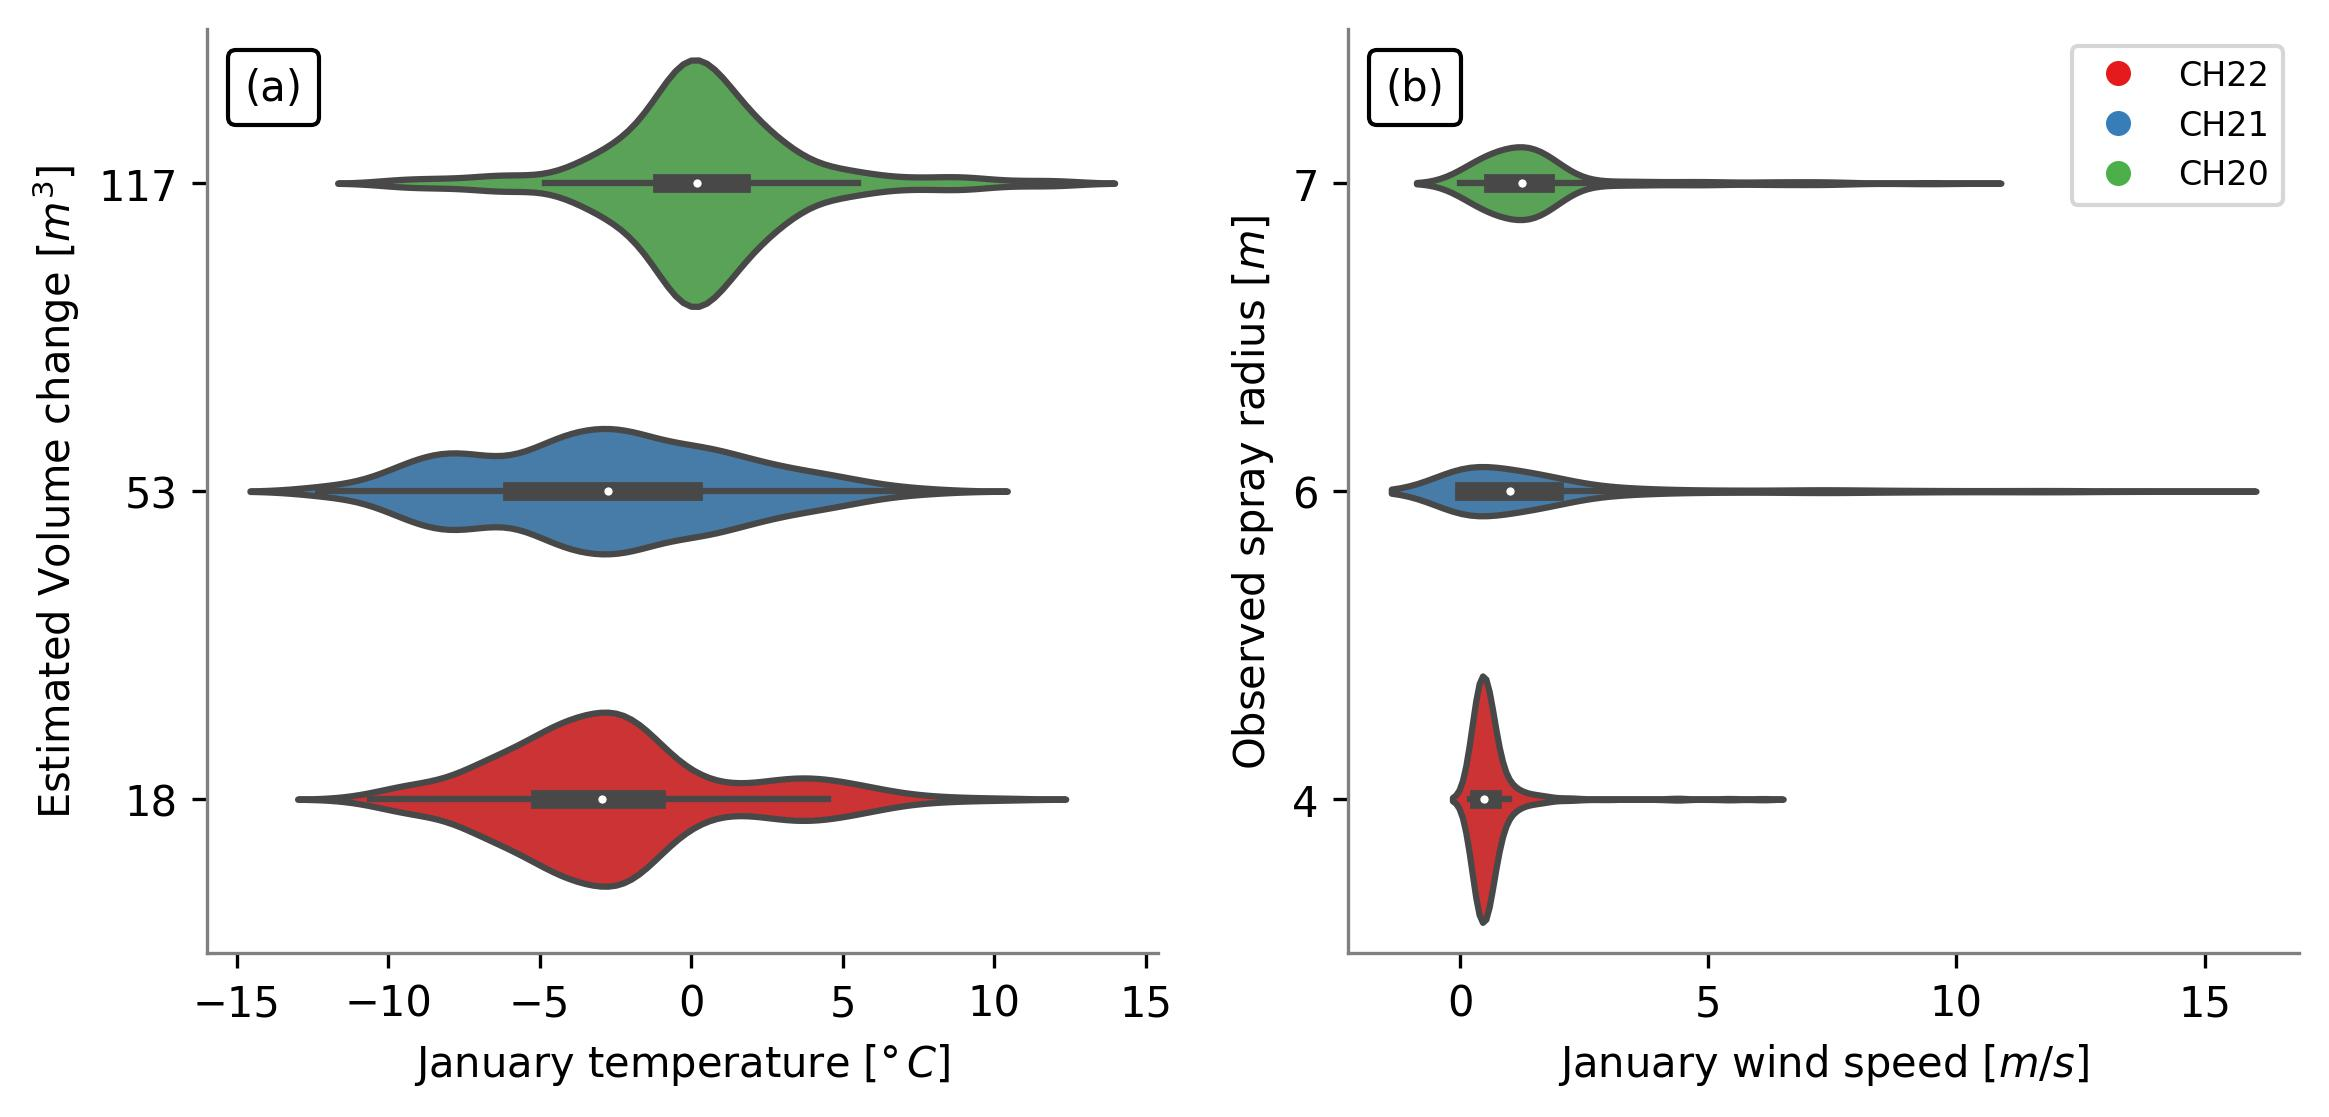
\includegraphics[width=\textwidth]{figs/CH_diffs.jpg}
\caption{(a) Estimated volume change and median temperature and (b) Observed spray radius and median wind speed
during january for AIRs built across three winters. } 
\label{fig:CH_diffs}
\end{figure}

\subsection{Interregional scale}

Comparison of AIR volume evolution show that Indian AIRs grew four times larger than Swiss AIRs (see Fig.
\ref{fig:2AIRs}). The corresponding freezing rate of the Indian AIR was more than ten times higher than the
Swiss. Sublimation was identified as the driving process of this difference (see paper II). Therefore, the
colder, drier and less cloudy weather characteristics of the Ladakh region made it more suitable to build AIRs
compared to the Guttannen region.

\begin{figure}[htb]
\centering
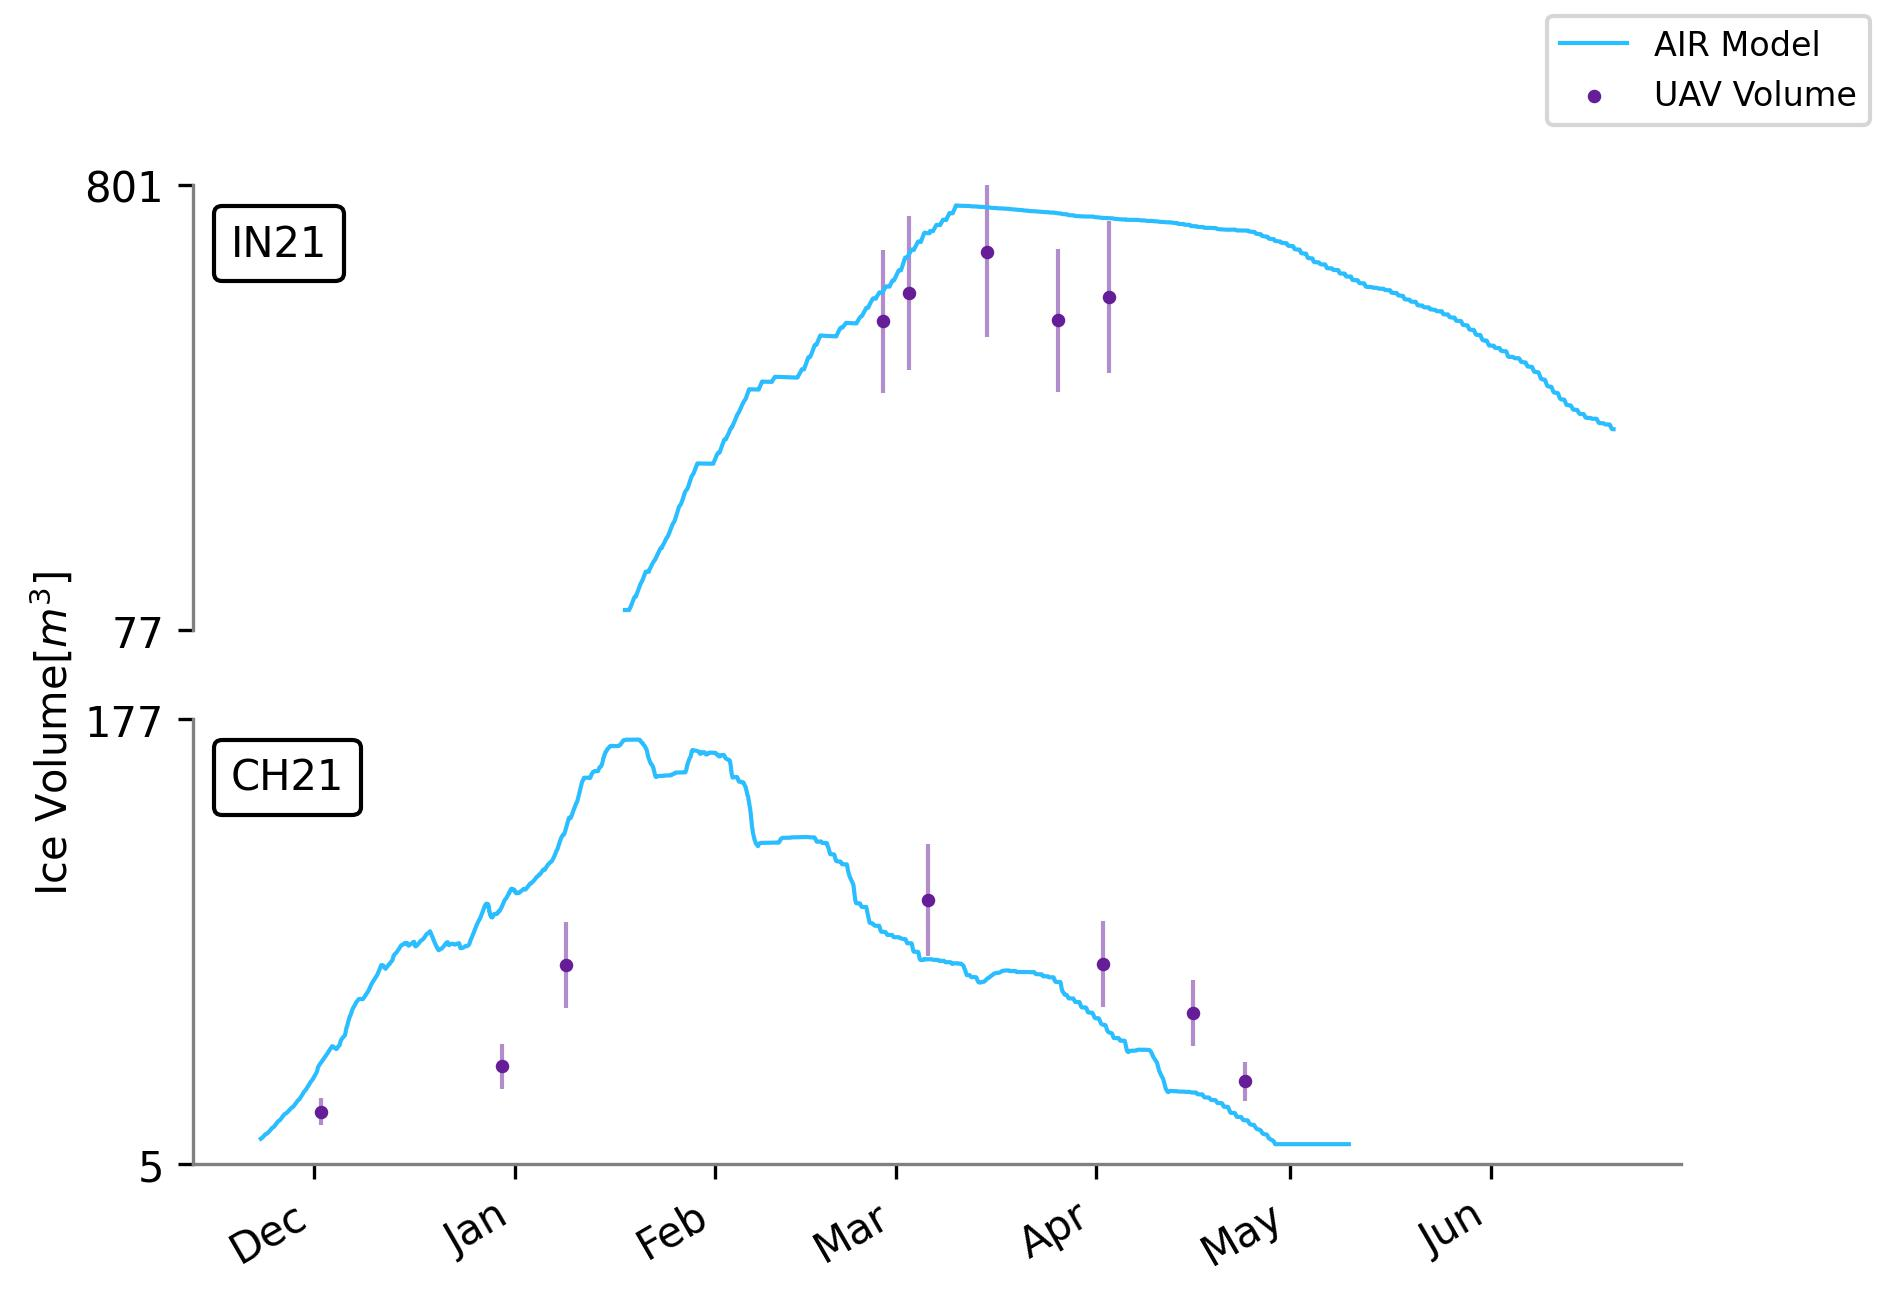
\includegraphics[width=12cm]{figs/IN21vsCH21.jpg}
\caption{AIRs show significant variation in volume evolution depending on the choice of construction location.}
\label{fig:2AIRs}
\end{figure}

\subsection{Intraregional scale}

\begin{figure}[htb]
	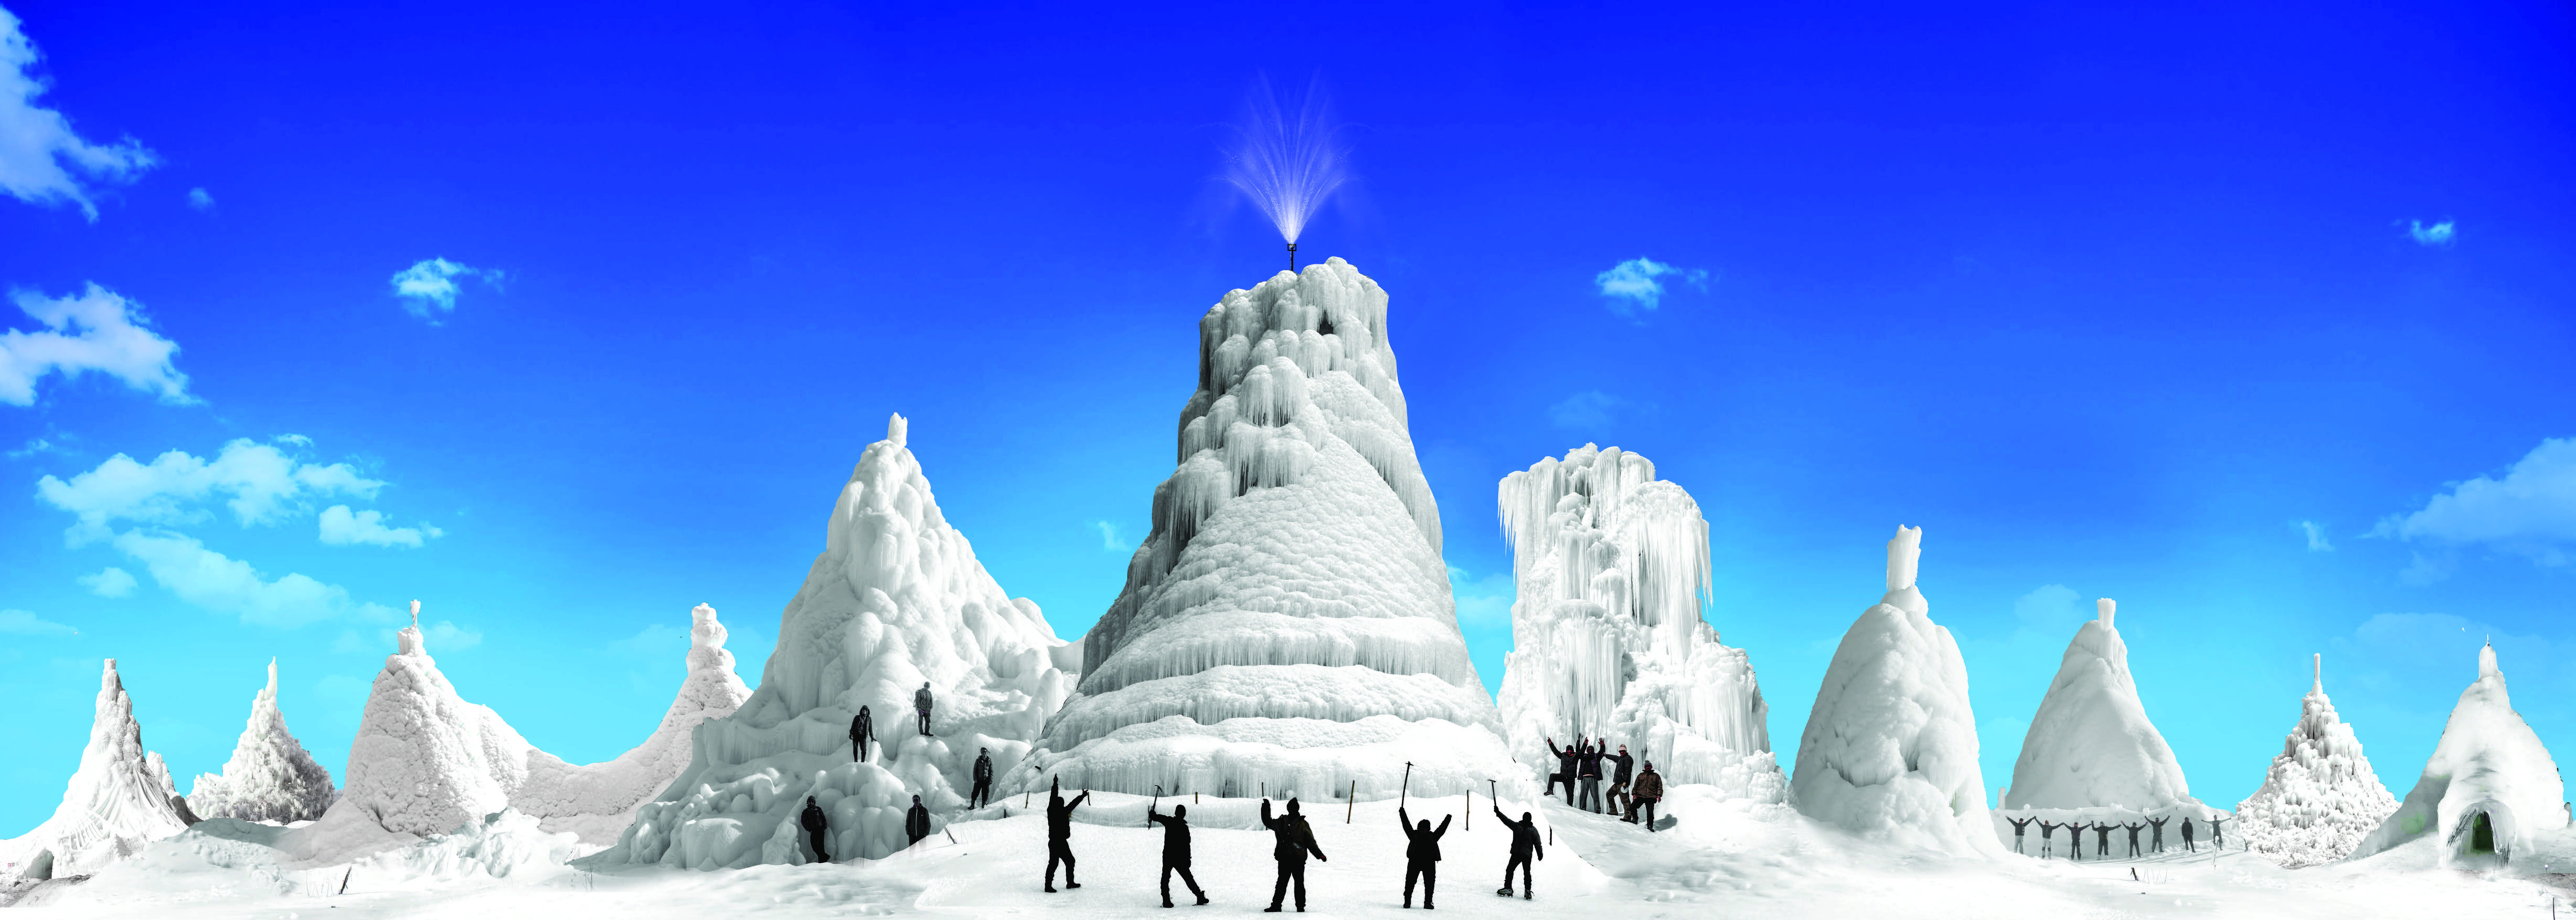
\includegraphics[width=\textwidth]{figs/AIRs_Ladakh}
	\caption{Compilation of AIRs built in different villages of Ladakh.}
	\label{fig:airs_ladakh}
\end{figure}

Regional AIR volume variation in Ladakh reveals a correlation of volume with the altitude of the construction
location (see Fig. \ref{fig:altvsvol}). However, higher altitude doesn't always yield higher volumes. This is
due to topographic effects of shadow valleys that reduce the sunshine hours of the location.

\begin{figure}[htb]
\centering
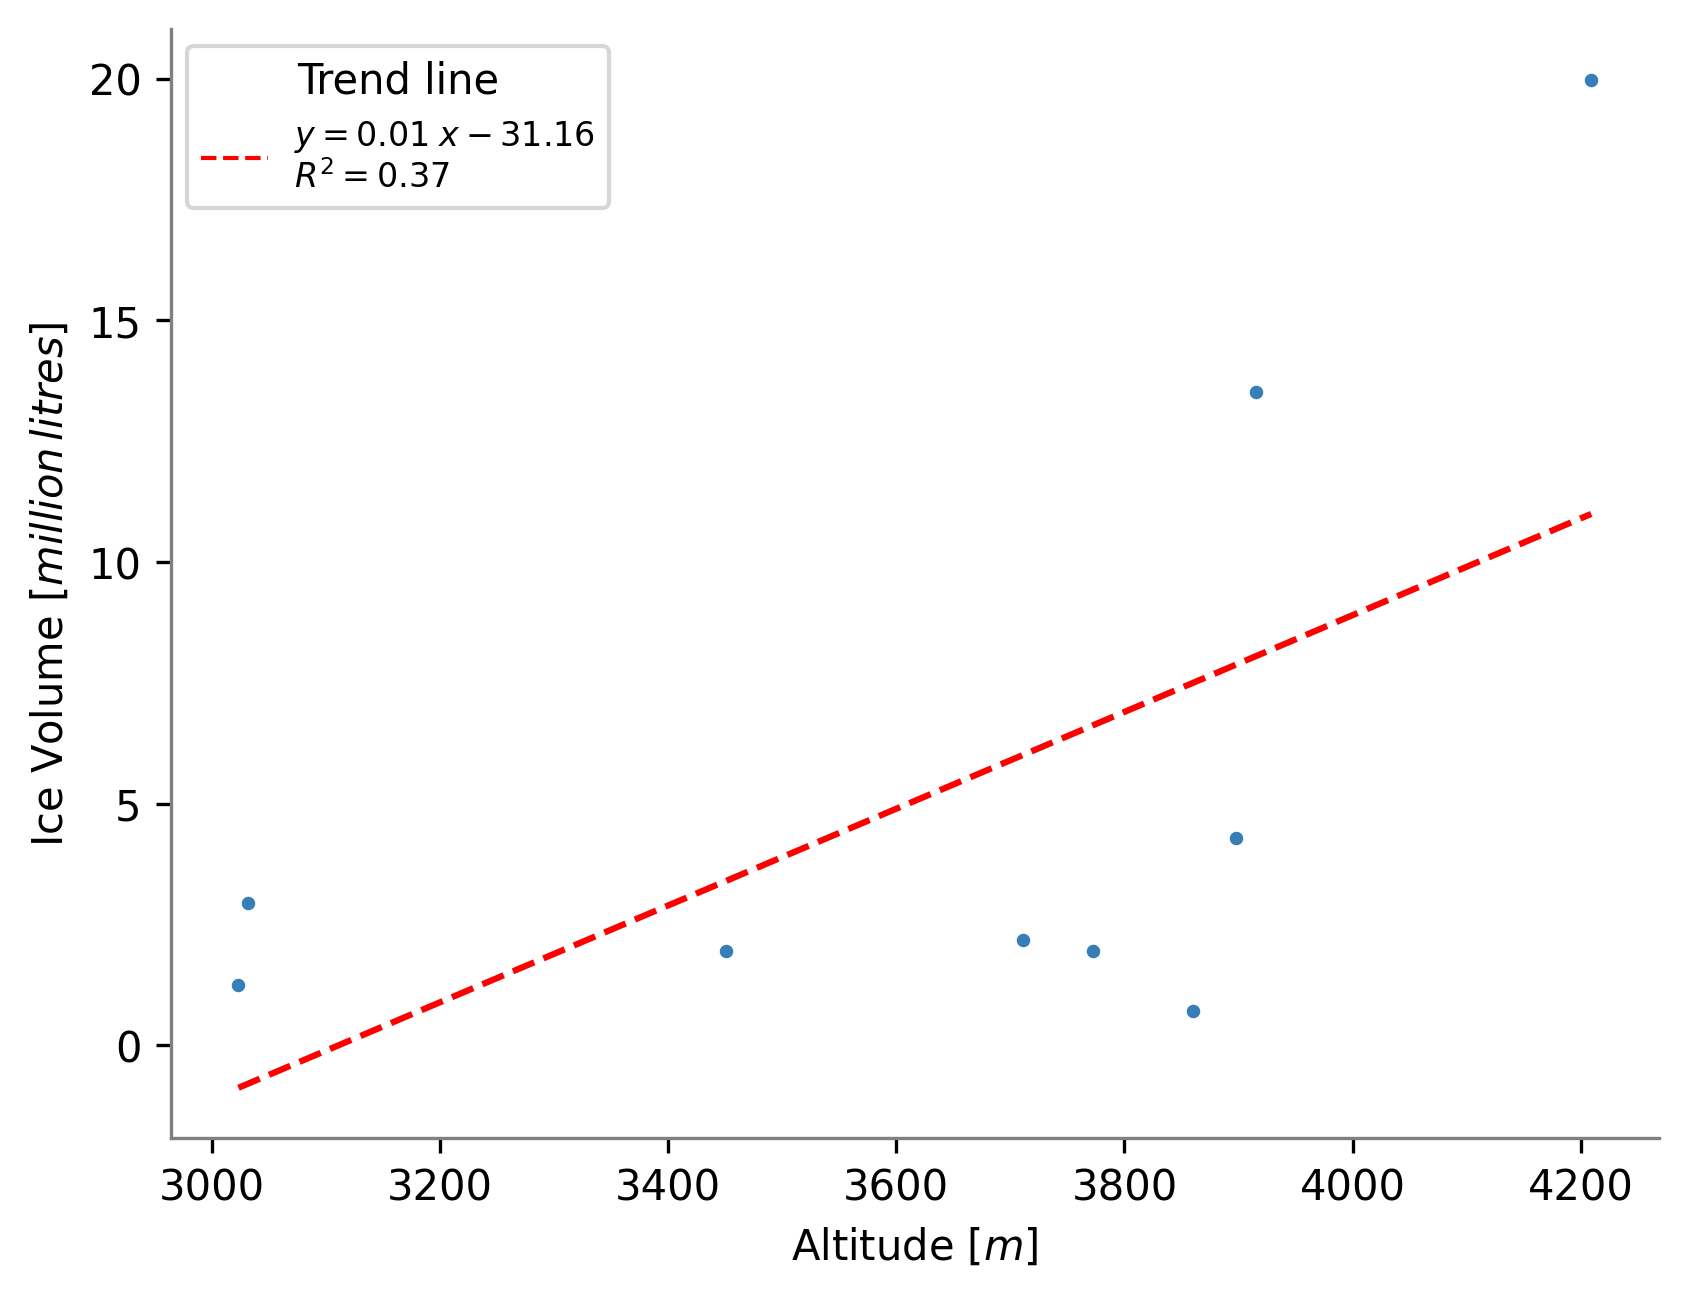
\includegraphics[width=12cm]{figs/altitudevsvolume.png}
\caption{(a) Estimated volume change and median temperature and (b) Observed spray radius and median wind speed
during january for AIRs built across three winters. }
\label{fig:altvsvol}
\end{figure}

\section{Metrics to judge site suitability}

Accordingly, we propose two sets of guidelines to constrain future construction sites in a regional and a local
scale. 

\subsection{Regional scale}

The values presented are determined based on past construction experiences and can be used as guidelines to
avoid construction attempts in unfavourable sites.

\begin{enumerate}

  \item Minimum median monthly temperature less than $0 \degree C$. 
  \item Water supply with median discharge rate more than $2\, l/min$.
  \item Terrain slope between water source and site greater than 10 m every km. 

\end{enumerate}

\subsection{Local scale}

Given a valley or a region satisfying the above requirements, further selection of sites around the particular
water supply can be performed using the criterions below: 

\begin{enumerate}
  \item Water source temperature is higher.
  \item Daylight hours are lower due to shadows.
  \item Altitude is higher.
\end{enumerate}

% Such villages are expected to produce AIRs that supply daily meltwater in the order of thousands of litres for 2
% months. 

% Different forms of AIRs show different sensitivities to each of these requirements. This is discussed in the
% next chapter.

% \subsection{Water supply}

% The water source of an AIR could be either a spring or a stream. Springs are the ideal water source since they
% are easy to transport via pipelines to the construction site due to their relatively warm temperatures. Other
% water sources have higher risks of freezing events in the fountain pipeline.

% \begin{itemize}
%   \item {\bf Water supply} : The water source of an AIR could be either a spring or a stream. Springs are the ideal
%     water source since they are easy to transport via pipelines to the construction site due to their relatively
%     warm temperatures. Other water sources have higher risks of pipeline freezing events. 

%   \item {\bf Weather conditions} : AIRs prefer colder, drier and less-cloudy regions. Correspondingly,
%     temperature, humidity and number of cloud-free days during the construction period can be used to rank
%     different sites. 

%   \item {\bf Topography} : AIRs prefer shadowed valleys. This is because these landforms have lower sunshine
%     hours which is the major driver of the melting rate of all the AIRs studied in this thesis.

% \end{itemize}

% This imposes several meteorological and topographical requirements for the chosen
% construction location. The meteorological requirements can be used to identify favourable regions worldwide
% whereas the topographical requirements can be used to pinpoint the construction site within the respective
% region. Below we detail these requirements and propose methodologies for finding construction sites satisfying
% them. 
  % \item Daylight hours are lower.
  % \item Cloudy days are lower.
  % \item Temperature is lower.
  % \item Humidity is lower.

% The ice reservoir technology has found limited adoption in regions beyond Ladakh. However, this

% It remains to be seen where else AIRs can be of utility.

% AIRs cannot be built anywhere. They require weather conditions cold enough to amass a seasonal stock of ice. The
% weather suitability of locations can be identified using the model developed in paper I. But such a methodology
% has a data requirement often incompatible with what is available. Reanalysis datasets like ERA5 can serve as 

% The utility of AIRs depends on their daily meltwater discharge. 

% Temperature based 

% AIRs exhibit significant interannual, interregional and intraregional volume variations depending on the
% suitability of the location 

% In this chapter, we attempt to quantify these requirements by examining the magnitude of these differences
% across the AIRs built in India and Switzerland. We also discuss strategies to judge the utility of AIRs in new
% locations.

% The spatial and temporal variation in weather conditions determine the growth rate of AIRs. In this section, we
% instead perform a qualitative analysis of the influence of interannual, interregional and intraregional
% variations in weather conditions on the AIR growth rate based on the Indian and Swiss AIR datasets.
